\documentclass[12pt,a4paper]{report}
\usepackage[margin=1in]{geometry}
\usepackage{titlesec}
\usepackage{amsmath}
\usepackage{amssymb}
\usepackage[colorlinks=true,urlcolor=black,linkcolor=black]{hyperref}
\usepackage{graphicx}
\usepackage{textcomp}
\usepackage{mathptmx}
\usepackage{tabto,enumitem}
\usepackage{algorithm}
\usepackage{algpseudocode}
\usepackage{wrapfig}

\titleformat{\chapter}{\bf\huge}{\thechapter}{20pt}{\huge\vspace{-.5em}}
    

\begin{document}

\begin{figure}
    \centering
    \begin{center}
    
\includegraphics[width=1.0\linewidth]{Images/cu_logo2.png}    
    \end{center}
    \label{fig:Concordia University Logo.}
\end{figure}

\title{SOEN 6011-Software Engineering Processes\\[3.0em] 

\text{Project Report on} \\
\textbf{Function 8 :\\  Standard Deviation ($\sigma$) } \\[2.5em] Submitted to:\\ Dr. Pankaj Kamthan}

\author{Aniket Tailor (40195068) }
\date{August 05, 2022}


\maketitle


\chapter{Problem no. 1}

\section*{Introduction}
The Standard Deviation is a measure of how spread out numbers are around the mean. It is denoted by Greek letter sigma $\sigma$. A low standard deviation implies that the data are grouped around the mean, whereas a large standard deviation shows that the data are more dispersed. In contrast, a high or low standard deviation indicates that the data points are, respectively, above or below the mean. A standard deviation that is close to zero implies that the data points are close to the mean.\\
\begin{equation*}
   (Standard Deviation) \quad \sigma = \sqrt\frac{{\Sigma (x- \overline{x})^2}}{n}
  \end{equation*}
  
Where:
    \begin{itemize}
        $\sigma$ = Standard Deviation\\
        $n$ = Size of the population\\
        $x$ = each value from population \\
        $\bar{x}$ = Mean of the population\\
    \end{itemize}

\section{Domain and Co-Domain}
\textbf{Domain:} Domain are the values which are given as input to the function. Hence in this case data values with natural and real numbers till infinity can be considered as domain.\\\\
\textbf{Co-Domain:} Co-Domain are the value which are given as output by the function. Therefore real numbers which are non negative and excluding imaginary numbers comes under Co-Domain. 

\section{Characteristics of Standard Deviation}
    \begin{itemize}[noitemsep]
        \item Only the spread or dispersion around a data set's mean is measured using the standard deviation.
        \item It can never be negative.
        \item The standard deviation is zero when all of the values in a data collection are the same because each value is equal to the mean.
        \item The higher the spread, the higher the standard deviation is for data with about the same mean.
        \item It is sensitive to outliers.
    \end{itemize}

\section{Context of Use Model}
\begin{figure}[h]
    \centering
    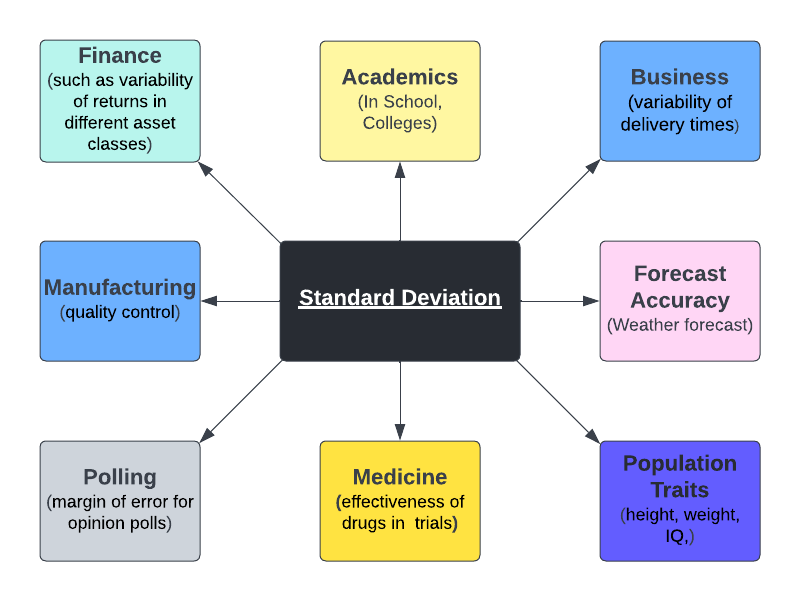
\includegraphics{Images/Context-of-use.png}
    \caption{Context of use model}
    \label{fig:Context of use model image}
\end{figure}

\chapter{Problem no. 2}
\section{Assumptions}
Any variable, as long as it can be sorted, can have its variance and standard deviation determined. However, the standard deviation is only a useful indicator of dispersion for a measurement variable when the data have a symmetrical distribution, which is frequently a normal distribution. If these presumptions are not true, using the standard deviation to show the variability of observations in range plots and box-and-whisker plots is misleading. This assumption is also a prerequisite for assumptions on the percentage of observations that fall within the range of agreement.

\section{Requirements}
\begin{enumerate}[noitemsep]
        \item \textbf{First Requirement}
        \begin{itemize}[noitemsep]
            \item \textbf{ID = } F1
            \item\textbf{Type = } Functional Requirement
            \item\textbf{Version = } 1.0
            \item\textbf{Priority = } High
            \item\textbf{Description = } Standard deviation only deals with numbers and not strings.
        \end{itemize}
        \item \textbf{Second Requirement}
        \begin{itemize}[noitemsep]
            \item \textbf{ID = } F2
            \item\textbf{Type = } Functional Requirement
            \item\textbf{Version = } 1.0
            \item\textbf{Priority = } High
            \item\textbf{Description = } Standard deviation is the square root of Variance, hence it's value should not be negative.
        \end{itemize}
        \item \textbf{Third Requirement}
        \begin{itemize}[noitemsep]
            \item \textbf{ID = } F3
            \item\textbf{Type = } Functional Requirement
            \item\textbf{Version = } 1.0
            \item\textbf{Priority = } Moderate
            \item\textbf{Description = }  The code should return correct sum of the input data values in order to find Standard Deviation
        \end{itemize}
        
        \newpage
        \item \textbf{Fourth Requirement}
        \begin{itemize}[noitemsep]
            \item \textbf{ID = } F4
            \item\textbf{Type = } Functional Requirement
            \item\textbf{Version = } 1.0
            \item\textbf{Priority = } High
            \item\textbf{Description = }   For calculating the mean, natural and real numbers should be considered.
        \end{itemize}
        \item \textbf{Fifth Requirement}
        \begin{itemize}[noitemsep]
            \item \textbf{ID = } F5
            \item\textbf{Type = } Functional Requirement
            \item\textbf{Version = } 1.0
            \item\textbf{Priority = } High
            \item\textbf{Description = }   For calculating standard deviation, at-least two numbers should be given as input.
        \end{itemize}
        \item \textbf{Sixth Requirement}
        \begin{itemize}[noitemsep]
            \item \textbf{ID = } F6
            \item\textbf{Type = } Functional Requirement
            \item\textbf{Version = } 1.0
            \item\textbf{Priority = } High
            \item\textbf{Description = }   If all the data values are same then the standard deviation should be 0.
        \end{itemize}
        \item \textbf{Seventh Requirement}
        \begin{itemize}[noitemsep]
            \item \textbf{ID = } NF7
            \item\textbf{Type = } Non Functional Requirement
            \item\textbf{Version = } 1.0
            \item\textbf{Priority = } Low
            \item\textbf{Description = }   Code should be well indented and easy to understand with proper documentation. 
        \end{itemize}
        \item \textbf{Eigth Requirement}
        \begin{itemize}[noitemsep]
            \item \textbf{ID = } NF8
            \item\textbf{Type = } Non Functional Requirement
            \item\textbf{Version = } 1.0
            \item\textbf{Priority = } Moderate
            \item\textbf{Description = }   Code should be portable that is a program running on windows 8 should run on windows 10 as well despite of change in performance. 
        \end{itemize}
        \newpage
    \end{enumerate}

\chapter{Problem no. 3}
\section*{Algorithms for Standard Deviation}
\textbf{1. Pseudo code of Traditional (Iterative) approach}\\

\begin{algorithm}
\caption{Traditional Algorithm}

\begin{algorithmic}[1]

\Procedure{StandardDeviation}{\;}
    \State $Sum \leftarrow 0$
    \State $Mean \leftarrow 0$
    \State $Var \leftarrow 0$
    \State $SD \leftarrow 0$
    \State $Number \leftarrow 0$
    \State $Size \leftarrow \;Array.count()$
    \State $Sum \leftarrow \;Sum+Sum$
    \For{$i \leftarrow 0,size$}
    \State $Sum+=Array$
    \EndFor
    \State $SD=squareRoot(SD/Size)$
    \State \textbf{Return} SD
    \EndProcedure
\Statex
\end{algorithmic}
\end{algorithm}

\section*{Which one to choose, Traditional or N-Pass?}
\begin{itemize}[noitemsep]
        \item Standard deviation can be calculated more quickly and with considerably more efficiency using the n-pass technique, which can accept more data inputs in the form of files. Other than that, the problem is that because it employs recursion rather than iteration, the memory stack would fill up quickly.
        \item The standard deviation can be calculated using the traditional approach, but it can take some time if the input data is huge and the frequency of the numbers is high. In addition, it is more prone to errors. As a result, the Multi pass or n-pass algorithm is more faster and more effective than the Traditional approach for standard deviation.

    \end{itemize}

\newpage
\section*{Algorithms for Standard Deviation}
\textbf{2. Pseudo code of N-Pass approach}\\
\begin{algorithm}
\caption{N-Pass Algorithm}
\begin{algorithmic}[1]

\Procedure{StandardDeviation}{\;}
    \State $Size \leftarrow \;Array.count()$
    \For{$i \leftarrow 0,size$}
    \State $Sum+=Array$
    \EndFor
    \State $Mean \leftarrow Sum/Size$
    \For{$i \leftarrow 0,size$}
    \State $SD=SD+power((Array[i]-Mean),2)$
    \EndFor
    \State $Variance=SD/Size$
    \State $SD=SquareRoot(Variance)$    
    \State \textbf{Return} SD
    \EndProcedure
\Statex
\Procedure{Power}{x,y}
    \For{$i \leftarrow 1,y$}
    \State $Result=Result*x$
    \EndFor
    \State \textbf{Return} Result
    \EndProcedure
\Statex
\Procedure{SquareRoot}{x}
    \State $temp$
    \State $sqrt \leftarrow \frac{x}{2}$
    \State $temp \leftarrow sqrt$
    \State $sqrt \leftarrow \frac{temp +\frac{x}{temp}}{2} $
    \While{$temp - sqrt \neq 0$}
    \State $temp \leftarrow sqrt$
    \State $sqrt \leftarrow \frac{temp +\frac{x}{temp}}{2} $
    \EndWhile
    \State \textbf{Return} $temp$
    \EndProcedure
\Statex
\end{algorithmic}
\end{algorithm}
\newpage
\section*{Mind Map}
The below given mind map shows the flow of the pseudo code for finding Standard Deviation. The algorithm will start from Main() method by taking input of data values. It will then call the CalculateSum() procedure to calculate sum of the data elements. With mean and array size in hand, CalculateVariance() method will be called. Internally this method calls Power() function to compute power and atlast SquareRoot() is used to find Standard Deviation.\\  
\begin{figure}[h]
    \centering
    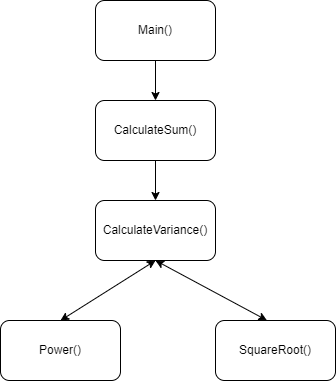
\includegraphics{Images/mindmap.png}
    \caption{Mind Map}
    \label{fig:Mind Map Image}
\end{figure}
\newpage
\section*{Pros of Traditional Algorithm}
\begin{itemize}
        \item This method does not uses the stack so it's faster.
        \item Traditional algorithm consumes less memory.
        \item The code is easy to understand and debug.
    \end{itemize}
\section*{Cons of Traditional Algorithm}
\begin{itemize}
        \item The iterative alternative is to repeatedly dynamically allocate or resize memory blocks. On many platforms automatic allocation is much faster, to the point that its speed bonus outweighs the speed penalty and storage cost of recursive calls.
        \item It makes the code longer.
        \item Sometimes execution and calculation time becomes higher.
    \end{itemize}
\section*{Pros of N-Pass Algorithm}
\begin{itemize}
        \item It is faster and much more efficient to use because it makes use of memory upto the mark. 
        \item Can take large set of data to find standard deviation.
        \item It makes the code smaller.

\end{itemize}
\section*{Cons of N-Pass Algorithm}
\begin{itemize}
        \item The inbuilt garbage collector begins to operate when the memory stack becomes mostly full, deleting the unused memory that has filled the stack.
\end{itemize}

\chapter{Problem no. 4}
\section{Error \& Exception Handling}

\begin{itemize}
    \item Error management makes it possible to gracefully handle both hardware and software problems and enables interrupted execution to continue. Either the programmer creates the necessary codes to handle problems or uses software tools to handle errors when it comes to error handling in software. When mistakes cannot be categorised, they are typically handled by returning unique error codes. For some applications, there exist specialised programs called error handlers that can assist in handling errors. These programs can foresee errors, assisting in recovery without actually terminating the program. 
    \item Responding to undesirable or unexpected events that occur while a computer program is running is known as exception handling. Without this process, exceptions would interfere with a program's regular functioning and cause it to crash. Exception handling deals with these events to prevent this from happening.
    \item In the given source code to find standard deviation, all the error and exception handling have been taken care of. To summarize a few exception handling errors, 
    \begin{enumerate}
        \item User cannot enter string as input. 
        \item If while entering the numerical data values, user enters a string by error then he/she will be prompted to enter the number again at that index value.
        \item User will need to re-enter the size of the array if it is 0.
        \item User should enter at-least two numbers, in order to find Standard Deviation.
        \item If all the elements of the array are same then it should given output as 0.
    \end{enumerate}
\end{itemize}

\newpage
\section{Debugger}
Debugging let you run a program interactively while keeping an eye on the variables and source code as they are being used. A break point in the source code indicates when the program's execution should halt while being fixed. Once the program has been paused, variables can be examined, their contents can be changed, etc. You can launch a Java program in Debug mode using Eclipse. Eclipse has a Debug viewpoint that offers you a ready-made selection of views. And through debug commands, Eclipse enables you to manage the execution flow.
\subsection{Advantages of debugger}
\begin{itemize}
    \item Debugging helps in solving the unknown problems in the code For example, compile time and run time exceptions.
    \item We can step into and out of the Eclipse debugger and check the dependencies of other variables with regard to the currently skipped variable.
    \item Debugging is a very useful tools for inspecting the state of the objects and variables in your code at run time.
\end{itemize}
\subsection{Disadvantages of debugger}
\begin{itemize}
    \item While in certain IDE's debuggers we can backtrack the debugger and examine its prior value, the Eclipse debugger does not allow us to do this.
    \item When multiple threads are active at once, debuggers frequently become stuck and refuse to advance.\\
    
\begin{figure}[h]
    \centering
    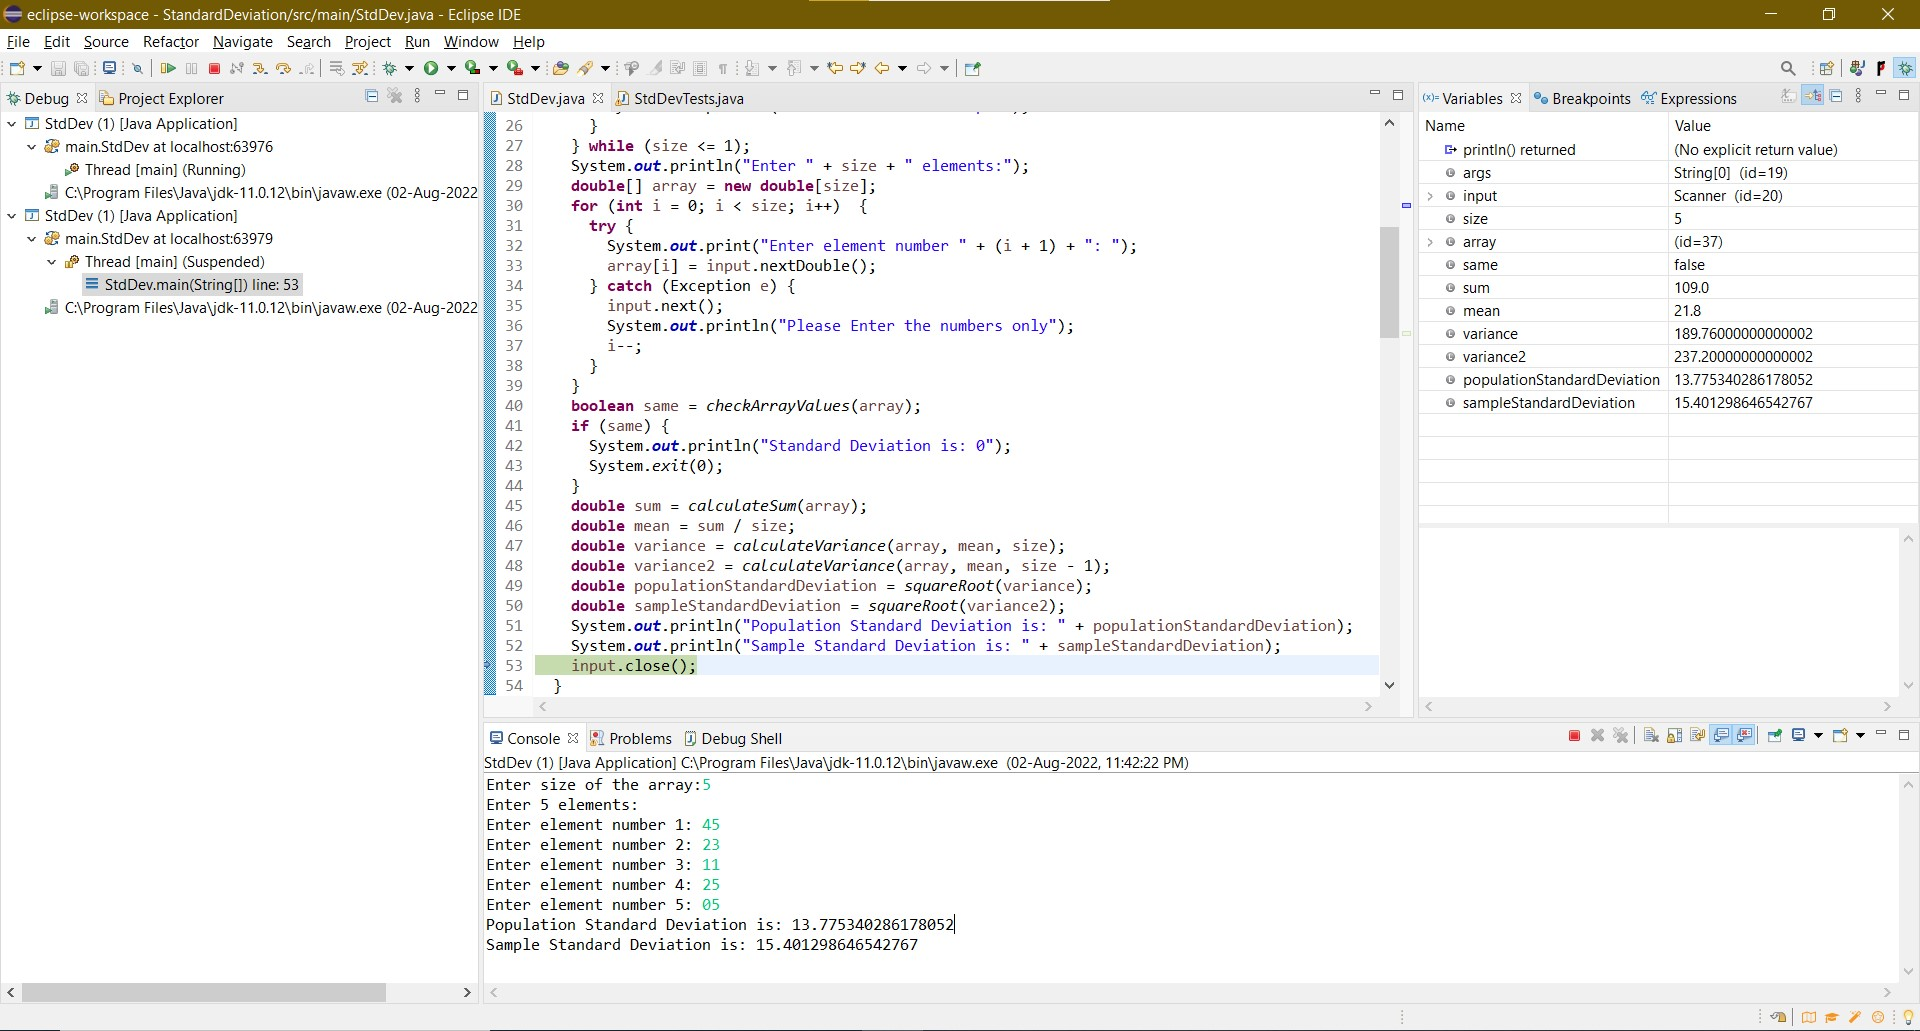
\includegraphics[width=0.90\linewidth]{Images/Debugger.jpg}
    \caption{Debugger in use}
    \label{fig:Debugger Image}
\end{figure}
\end{itemize}

\newpage
\section{Checkstyle}
Programmers can use Checkstyle as a development tool to write Java code that follows a coding standard. To relieve humans of this tedious work, it automates the process of checking Java code. It is therefore perfect for initiatives that aim to impose a coding standard. It may examine a variety of elements in your source code. It can identify issues with class and method design. It can also check for formatting and code layout problems.
\subsection{Advantages of Checkstyle}
\begin{itemize}
    \item Portable between IDEs [Eclipse And IntelliJ]
    \item Due to the fact that check style was truly intended to be an independent framework, integrating it with your external tools is considerably simpler.
    \item It lets you format the code with respect to global standards. 
    \item Ability of creating your own rules. Eclipse defines a large set of styles, but checkstyle has more, and you can add your own custom rules.

\end{itemize}
\subsection{Disadvantages of Checkstyle}
\begin{itemize}
    \item Removes the ability to do any 'special-case' formatting where an alternate format would make code more readable.
    \item The checks done by checkstyle do not confirm the correctness or completeness of the code.
    \item It ties you into using IDEs which support exactly the reformatting features you need.
    
\begin{figure}[h]
    \centering
    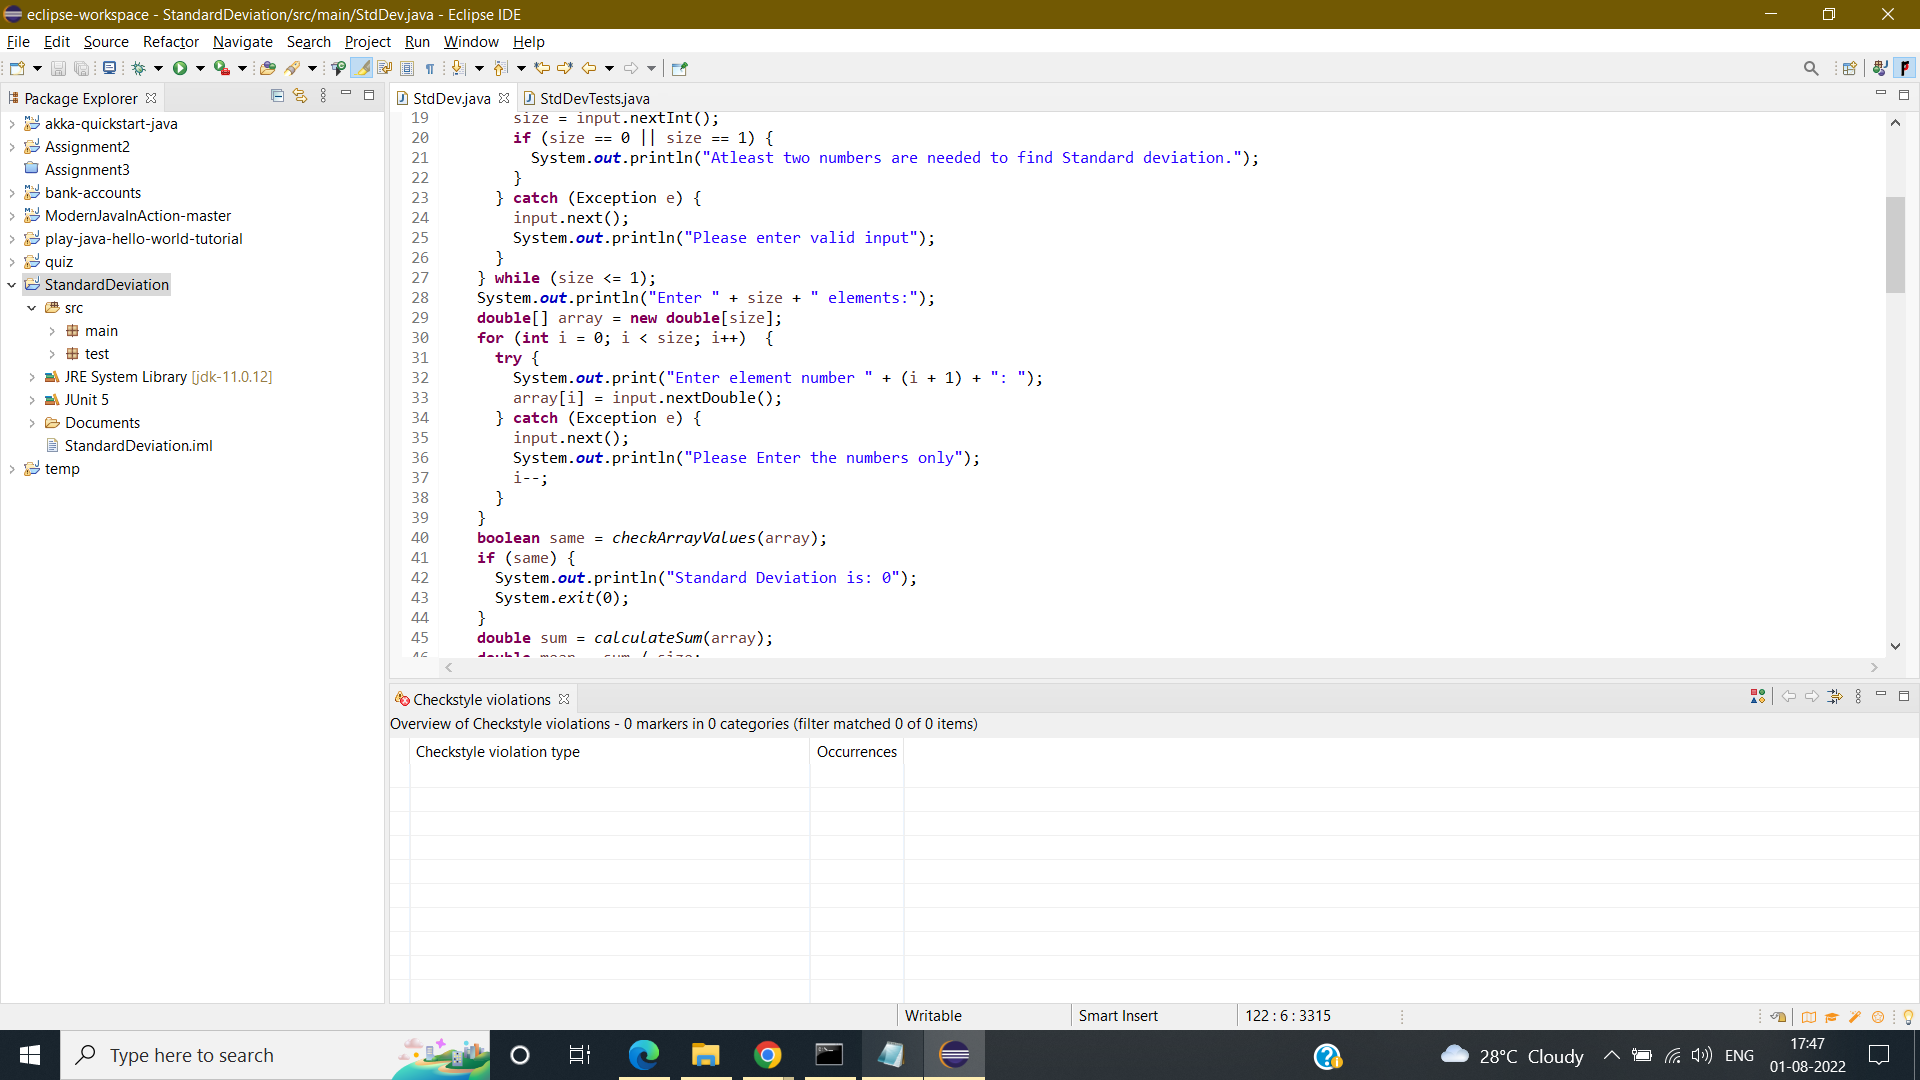
\includegraphics[width=0.87\linewidth]{Images/Checkstyle.png}
    \caption{Checkstyle in use}
    \label{fig:Checkstyle Image}
\end{figure}
\end{itemize}

\chapter{Problem no. 5}
\section{Requirements Traceability}
In this section, all the unit tests are traced with the requirements from Problem 2. Unit testing is done using the JUnit framework of Java. 

\subsection*{Test Case number 1}
    \begin{itemize}
        \item \textbf{Test Case ID: } UTC1
        \item \textbf{Corresponding Requirement ID: } F3, F4
        \item \textbf{Test Case Method: } testCalculateSum()
        \item \textbf{Description: } The testCalculateSum(), as the name suggests it verifies if the CalculateSum() method is calculating the total of all the array elements as expected. 
    \end{itemize}
    
\subsection*{Test Case number 2}
    \begin{itemize}
        \item \textbf{Test Case ID: } UTC2
        \item \textbf{Corresponding Requirement ID: } F2
        \item \textbf{Test Case Method: } testPower()
        \item \textbf{Description: } The testPower() method, verifies if the Power() method is returning the correct power of a number. 
    \end{itemize}
    
\subsection*{Test Case number 3}
    \begin{itemize}
        \item \textbf{Test Case ID: } UTC3
        \item \textbf{Corresponding Requirement ID: } F2, F4
        \item \textbf{Test Case Method: } testCalculateVariance()
        \item \textbf{Description: } The testCalculateVariance() method tests the calculateVariance() method in the source code. It makes sure if the responsible method is working fine and calculating variance as expected. 
    \end{itemize}
    
\subsection*{Test Case number 4}
    \begin{itemize}
        \item \textbf{Test Case ID: } UTC4
        \item \textbf{Corresponding Requirement ID: } F2
        \item \textbf{Test Case Method: } testSquareRoot()
        \item \textbf{Description: } This method verifies the squareRoot() method in source code. As the name goes it checks the square root of a number. 
    \end{itemize}

\subsection*{Test Case number 5}
    \begin{itemize}
        \item \textbf{Test Case ID: } UTC5
        \item \textbf{Corresponding Requirement ID: } F1, F5, NF7
        \item \textbf{Test Case Method: } testMain()
        \item \textbf{Description: } The testMain() method tests out driver function (Main). It tests the main() function with all different types of inputs such as String, Real numbers, Whole numbers. If any inappropriate input is given then proper error and exception handling is in place. It won't let the program terminate or crash. 
    \end{itemize}
    
\subsection*{Test Case number 6}
    \begin{itemize}
        \item \textbf{Test Case ID: } UTC6
        \item \textbf{Corresponding Requirement ID: } F6
        \item \textbf{Test Case Method: } testMainSameValues()
        \item \textbf{Description: } When all the array elements are same, at that time the Standard Deviation turns out to be 0. Hence this unit test case checks the scenario where all the input values are same. 
    \end{itemize}
    
\begin{thebibliography}{15}

\addcontentsline{toc}{chapter}{Bibliography}
\bibitem{1}
\href{https://en.wikipedia.org/wiki/Standard_deviation}{https://en.wikipedia.org/wiki/Standard\_deviation}

\bibitem{2}
\href{https://www.investopedia.com/terms/s/standarddeviation.asp}{https://www.investopedia.com/terms/s/standarddeviation.asp}

\bibitem{3}
\href{https://www.nlm.nih.gov/nichsr/stats\_tutorial/section2/mod8\_sd.html}{https://www.nlm.nih.gov/nichsr/stats\_tutorial/section2/mod8\_sd.html}

\bibitem{4}
\href{https://benpfaff.org/writings/clc/recursion-vs-iteration.html#:~:text=The\%20iterative\%20alternative\%20is\%20to,storage\%20cost\%20of\%20recursive\%20calls.}{https://benpfaff.org/writings/clc/recursion-vs-iteration.html}

\bibitem{5}
\href{https://www.tutorialspoint.com/what-are-the-differences-between-recursion-and-iteration-in-java}{https://www.tutorialspoint.com/what-are-the-differences-between-recursion-and-iteration-in-java}

\bibitem{6}
\href{https://influentialpoints.com/Training/variance_and_standard_deviation-principles-properties-assumptions}{https://influentialpoints.com/Training/variance\_and\_standard\_deviation-principles-properties-assumptions}

\bibitem{7}
\href{https://www.techtarget.com/searchsoftwarequality/definition/error-handling}{https://www.techtarget.com/searchsoftwarequality/definition/error-handling}

\bibitem{8}
\href{https://www.techopedia.com/definition/16626/error-handling}{https://www.techopedia.com/definition/16626/error-handling}

\bibitem{9}
\href{https://checkstyle.sourceforge.io/}{https://checkstyle.sourceforge.io/}

\bibitem{10}
\href{https://softwareengineering.stackexchange.com/questions/92256/advantages-and-disadvantages-of-forced-code-reformat}{https://softwareengineering.stackexchange.com/questions/92256/advantages-and-disadvantages-of-forced-code-reformat}

\end{thebibliography}
\end{document}